%%%%%%%%%%%%%%%%%%%%%%%%%%%%%%%%%%%%%%%%%%%%%%%%%%%%%%%%%%%%%%%%%%%%%%%%%%%
%% This file is part of the book
%%
%% Algorithmic Graph Theory
%% http://code.google.com/p/graph-theory-algorithms-book/
%%
%% Copyright (C) 2009, 2010 Minh Van Nguyen <nguyenminh2@gmail.com>
%%
%% See the file COPYING for copying conditions.
%%%%%%%%%%%%%%%%%%%%%%%%%%%%%%%%%%%%%%%%%%%%%%%%%%%%%%%%%%%%%%%%%%%%%%%%%%%

%% breadth-first searching the Petersen graph
\subfigure[Breadth-first search.]{
\index{breadth-first search}
\index{Petersen graph}
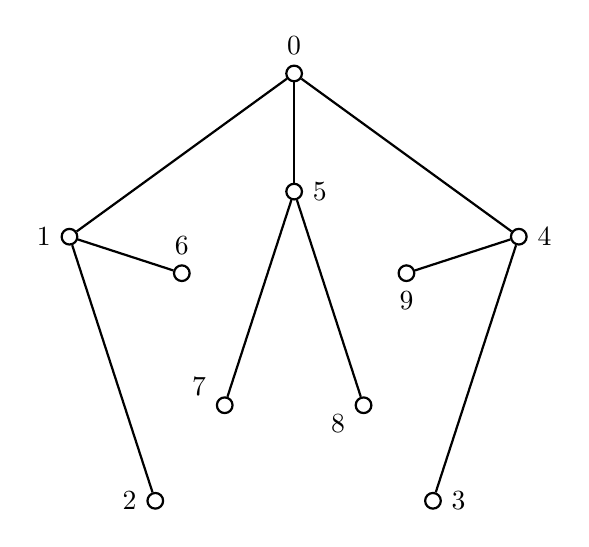
\begin{tikzpicture}
[nodedecorate/.style={shape=circle,inner sep=2pt,draw,thick},%
  linedecorate/.style={-,thick},
  scale=1.5]
%% nodes or vertices
\foreach \nodename/\x/\y/\direction/\navigate in {
  %% inner star
  5/0.0/1.0/right/east, 9/0.9510/0.3090/below/south,
  8/0.5877/-0.8090/below left/west, 7/-0.5877/-0.8090/above left/west,
  6/-0.9510/0.3090/above/north,
  %% outer pentagon
  0/0.0/2.0/above/north, 4/1.9021/0.6180/right/east,
  3/1.1755/-1.6180/right/east, 2/-1.1755/-1.6180/left/west,
  1/-1.9021/0.6180/left/west}
{
  \node (\nodename) at (\x,\y) [nodedecorate] {};
  \node [\direction] at (\nodename.\navigate) {$\nodename$};
}
%% edges or lines
\path
\foreach \startnode/\endnode in {0/1, 0/4, 0/5, 1/2, 1/6, 4/3, 4/9,
  5/7, 5/8}
{
  (\startnode) edge[linedecorate] node {} (\endnode)
};
\end{tikzpicture}

}
\quad
%%
%% depth-first searching the Petersen graph
\subfigure[Depth-first search.]{
\index{depth-first search}
\index{Petersen graph}
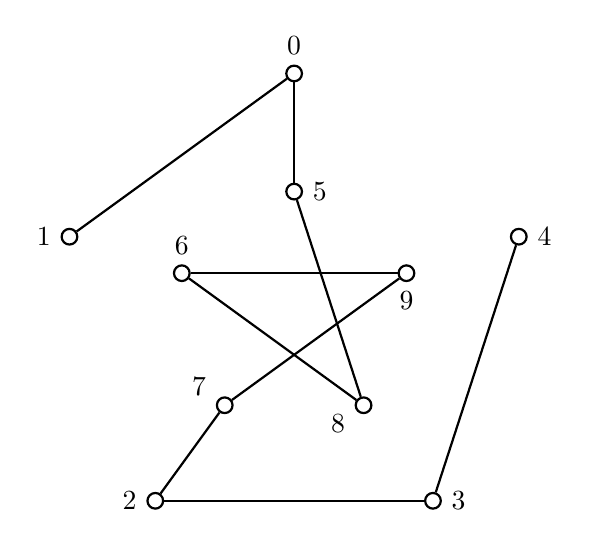
\begin{tikzpicture}
[nodedecorate/.style={shape=circle,inner sep=2pt,draw,thick},%
  linedecorate/.style={-,thick},
  scale=1.5]
%% nodes or vertices
\foreach \nodename/\x/\y/\direction/\navigate in {
  %% inner star
  5/0.0/1.0/right/east, 9/0.9510/0.3090/below/south,
  8/0.5877/-0.8090/below left/west, 7/-0.5877/-0.8090/above left/west,
  6/-0.9510/0.3090/above/north,
  %% outer pentagon
  0/0.0/2.0/above/north, 4/1.9021/0.6180/right/east,
  3/1.1755/-1.6180/right/east, 2/-1.1755/-1.6180/left/west,
  1/-1.9021/0.6180/left/west}
{
  \node (\nodename) at (\x,\y) [nodedecorate] {};
  \node [\direction] at (\nodename.\navigate) {$\nodename$};
}
%% edges or lines
\path
\foreach \startnode/\endnode in {0/5, 5/8, 8/6, 6/9, 9/7, 7/2, 2/3,
  3/4, 0/1}
{
  (\startnode) edge[linedecorate] node {} (\endnode)
};
\end{tikzpicture}
}
